\section{Training and First Experiments}\label{sec:fcat-expe}
% training process
We use the training process schematized in \cref{fig:fcat-training} to train our intent generation model on the dataset used for BoA.
For details on the data, refer back to \cref{sec:boa-training-data}.
We train the intent model with BCE on the intent matrix and the cover and order relation.
We also use MSE between the generated intent embeddings and the expected intent embeddings, produced by applying the object embedding process of BoA on the intent matrix.
Using MSE on the expected intent embedding has proven, experimentally, to improve the performance and convergence speed compared to using only the BCE on the intent matrix.
We also confirmed that the intent prediction performance was not hindered by the BCE for the order and cover relations.
Finally, retraining the BoA decoder with the rest of the model converges faster but performs worse than training only the intent model.

\begin{figure}
\centering
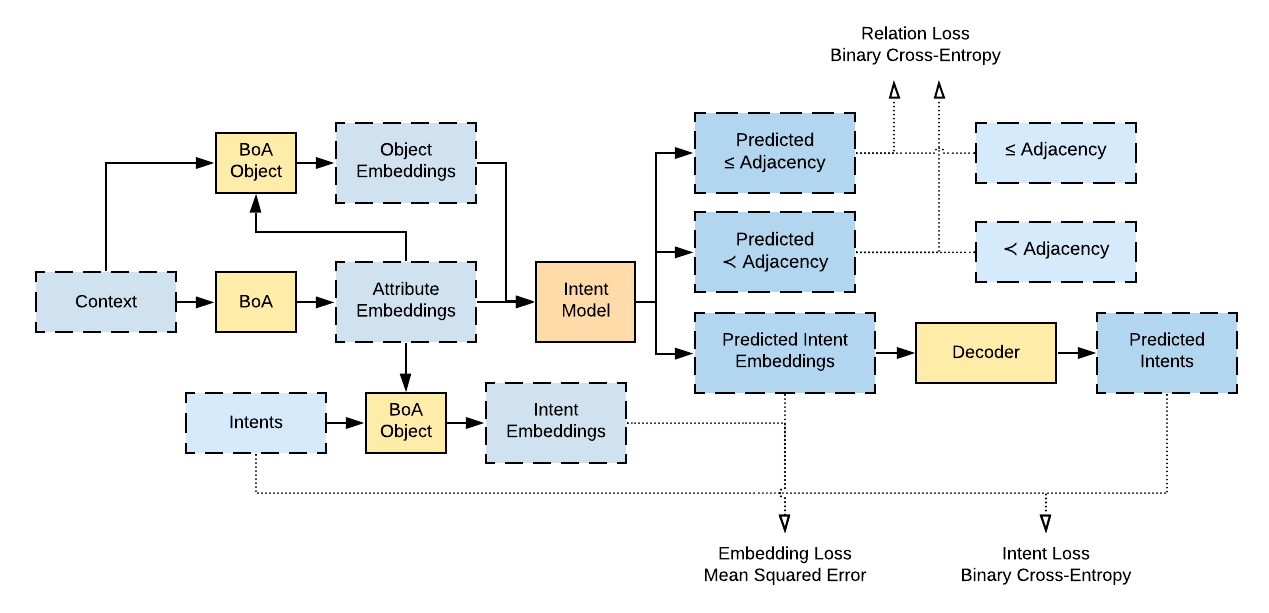
\includegraphics[height=12cm, width=\textwidth, keepaspectratio]{Figures/Ch3/fcat_training.png}
\caption{Schematic representation of the intent model training process.} \label{fig:fcat-training}
\end{figure}

We rely on two sets of measures to evaluate the performance of our model for intent generation.
First, we determine the predictive performance at the scale of each component of the intent matrix using AUC ROC.
%Then, we determine the best threshold using the ROC and apply it on the intent matrix.
Then, we apply a threshold of $0.5$ on the intent matrix.
We transform the resulting matrix into a set of predicted intents $\hat{I}$, so we remove all duplicate predicted intents.
After removing the duplicates from the set versions of the intents, we compute the intent precision as ${|\hat{I}\cap I|}/{|\hat{I}|}$ and the recall as ${|\hat{I}\cap I|}/{|I|}$. From the precision and recall we can compute the F1 score.
%
We also use the AUC ROC to measure the prediction performance on the relation prediction by the attention, for both $\leq$ and $\prec$.
We apply it on the adjacency vector of the relations, as described in \cref{sec:enc-adjacency}.

We report the performance on our evaluation set in \cref{tab:fcat-perf}, and show the prediction result for a few samples of the training set in \cref{fig:fcat-perf}.
The model presented was trained for 12h which corresponds to 50 epochs.
The AUC ROC for the two relations $\leq$ and $\prec$ is close to $0.85$ which is not perfect but not bad either.
However, the AUC ROC on the intent matrix is $0.72$, which is still above a random model but is not good enough for our application.
Indeed, the precision on the intents is under 25\% in average, and the recall and F1 are under 10\%.
The qualitative results displayed in \cref{fig:fcat-perf} are better than the ones obtained in the preliminary experiments.
It is interesting to note that for the first of the two samples, the first 50 predicted concepts look similar and are processed similarly by the attention generating the order relation, resulting in a slightly denser column between 0 and 50 in the adjacency of $\leq$ (\nth{6} column of the picture. This indicates that the intent and the relations are related within the model.


\begin{table}[t]
\centering
\begin{tabular}{rr}
\toprule
Measure & Mean $\pm$ std. \\
\midrule
Intent precision              & $ 0.217\pm 0.224 $ \\
Intent recall                 & $ 0.071\pm 0.092 $ \\
Intent F1                     & $ 0.046\pm 0.054 $ \\
%Intent miss rate              & $ 0.929\pm 0.092 $ \\
%Intent false discovery rate   & $ 0.783\pm 0.224 $ \\
\midrule
Intent matrix AUC ROC & $ 0.720\pm 0.062 $ \\
$\leq$ AUC ROC        & $ 0.852\pm 0.071 $ \\
$\prec$ AUC ROC       & $ 0.846\pm 0.072 $ \\
\bottomrule
\end{tabular}
\caption{Performance of the intent model on the evaluation set.}\label{tab:fcat-perf}
\end{table}

\begin{figure}
    \centering
    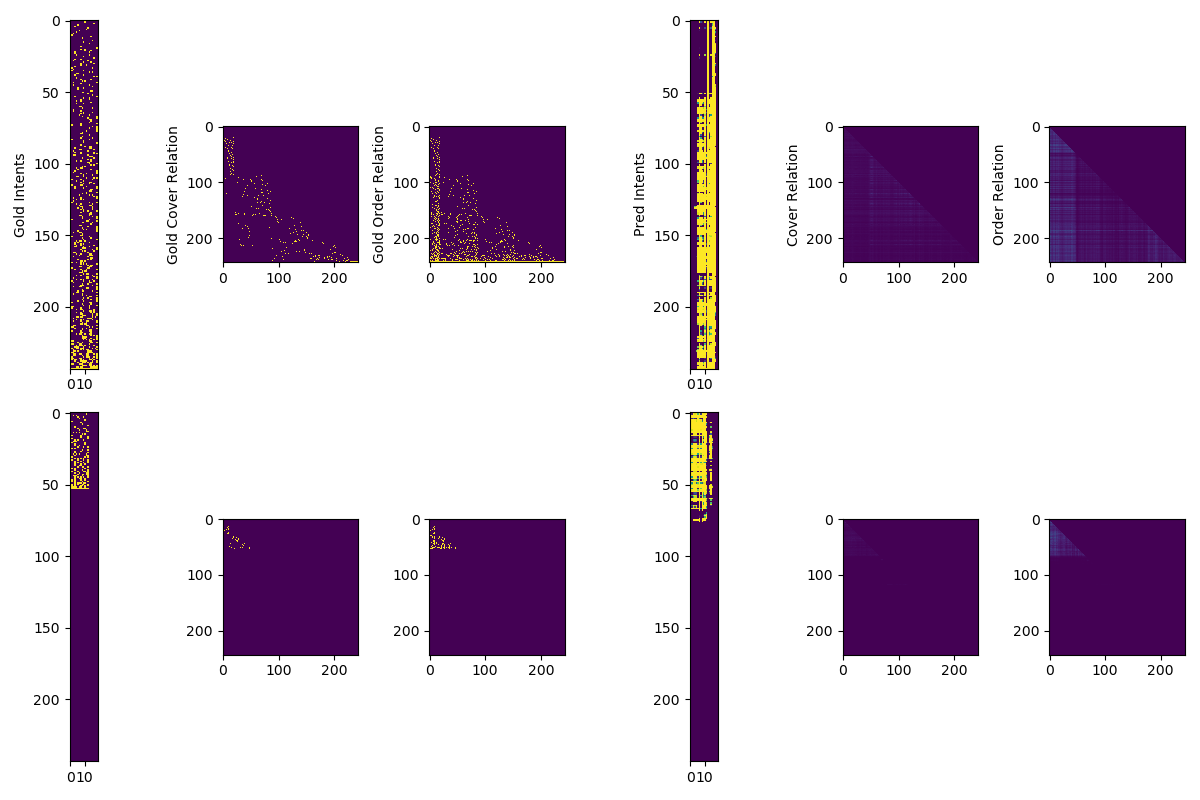
\includegraphics[keepaspectratio, width=.9\textwidth]{Figures/Ch3/concept_small.png}
    \caption{Batch of 2 samples (one per row) of the evaluation set and the predictions of our model. The first three columns correspond to the sample itself, and the last three to the model's prediction.}
    \label{fig:fcat-perf}
\end{figure}